\subsection{Der Rulebase-Manager}
\label{sec:rbmanager}

Generierte Erkennungsregeln können mit Hilfe des \textit{Rulebase Manager} verwaltet werden (vgl. Abb. \ref{silif-rulebase_manager}).

\begin{figure}[H]
\centering
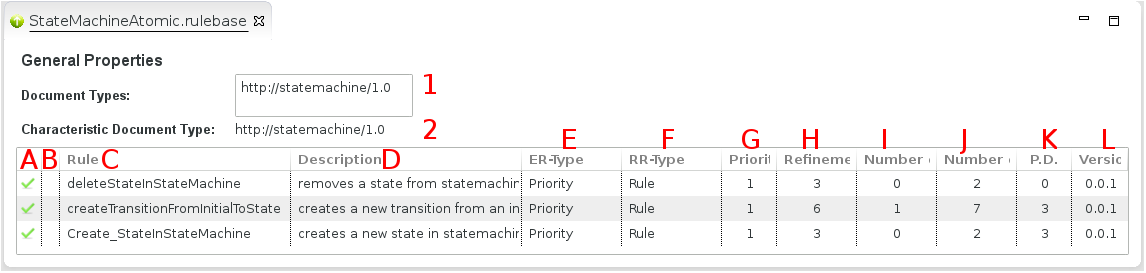
\includegraphics[width=0.8\textwidth]{recognitionrules/graphics/silift-rulebase_manager.png}
\caption{Erstellen eines \textit{Rulebase Manager}}
\label{silif-rulebase_manager}
\end{figure}

\begin{enumerate}
	\item Dokumenttypen der Regelbasis.
	\item Karakterisierender Dokumenttyp der Regelbasis.
\end{enumerate}

\begin{enumerate}[(A)]
\item Durch Klicken auf das Häkchen können einzelne Erkennungsregeln für die \textit{Recognition-Engine} aktiviert (grün) bzw. deaktiviert (grau) werden.

\item Zeigt an ob die zugehörige Editierregel valide ist. Sofern die Regel invalide ist wird ein Fehlersymbol angezeigt. Durch Klicken auf das Symbol wird der Validierungsfehler angezeigt.

\item Repräsentiert den Verwaltungsname der Editier-, bzw. Erkennungsregel. Dieser kann durch den Rulebase Manager editiert werden, wird aber nur zur Anzeige in der GUI verwendet.

\item Beschreibung der Editier-, bzw. Erkennungsregel.

\item Henshin Typ der \textit{mainUnit} der Editierregel (\texttt{Independent}, \texttt{Priority}, \texttt{Sequential} usw.).

\item Henshin Typ der Erkennungsregel (Rule und Multi-Rule).

\item Priorität der Erkennungsregel:
 Gerade unter zusätzlicher Verwendung komplexer Editierregeln kann es vorkommen, dass zwei Semantic Change Sets (vgl. \pageref{page:semantic_change_sets}) die gleichen low-level-Änderungen beinhalten. 
Für den Fall kann man einer Regel eine höhere Priorität zuordnen. 

\item \textit{Refinement-Level}: 
Für den Fall, dass auch die Prioritäten zweier identischer Semantic Change Sets gleich sind, versucht SiLift anhand der Anzahl der Supertypen die "'speziellere"' Regel zu bestimmen. 
D.h. je mehr Supertypen die Knoten der Regel besitzen, desto spezieller ist diese. 

\item Anzahl der positiven und negativen Application Conditions (PACs/NACs).

\item Anzahl der Parameter der Erkennungsregel.

\item \textit{Potential Dependicies}: 
Anzahl der potentiellen Abhängigkeiten zu anderen Editieroperationen. 
Das sequentielle Ausführen mehrere Editieroperationen ist nicht kommutativ, d.h. es können zwischen den jeweiligen Editieroperationen Abhängigkeiten existieren, die beim generieren eines Patches berücksichtigt werden müssen. 

\item Version der Erkennungsregel.
\end{enumerate}

I.d.R. wächst eine Regelbasis mit der Zeit. 
Es ist so gut wie unmöglich alle möglichen Editieroperationen im Vorfeld aufzudecken und zu implementieren. 
Um Ihrer bestehenden Regelbasis neue Regeln hinzuzufügen klicken Sie auf \texttt{Generate new recognition rules} (vgl. Abb. \ref{silift-rulebase_manager_create_new_rules}) und wählen die entsprechenden Editierregeln aus. 
Die abgeleiteten Erkennungsregeln werden nun der bestehenden Regelbasis hinzugefügt.

\begin{figure}[H]
\centering
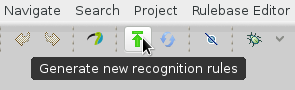
\includegraphics[width=0.25\textwidth]{recognitionrules/graphics/silift-rulebase_manager_create_new_rules.png}
\caption{Erkennungsregeln einer bestehenden \textit{Rulebase} hinzufügen}
\label{silift-rulebase_manager_create_new_rules}
\end{figure}
